\documentclass[a4paper]{article}
\usepackage{lipsum}
\usepackage{graphicx} % Required for inserting images
\usepackage{multicol}
\usepackage{amssymb}
\usepackage{enumitem}

\usepackage{blindtext}
\usepackage{indentfirst}
\usepackage[hyphenbreaks]{breakurl}
\usepackage[hyphens]{url}%позволяет переносить сылки
\usepackage{enumerate}%позволяет делать маркеровку в списке
\usepackage{biblatex}%импортирует пакет
\addbibresource{sample.bib}%импортирует сам файл
\bibliography{25}
\usepackage{amsmath,amssymb}
\usepackage[english,russian]{babel}




\usepackage[%
left=0.50in,%
right=0.50in,%
top=0.5in,%
bottom=1.0in,%
left=0.50in,%
paperheight=11in,%
paperwidth=7.4in,%
]{geometry}%
\newcommand{\Rn}[1]{\Roman numeral#1\relax}
\newcommand{\RN}[1]{\uppercase\expandafter{\Roman numeral#1}}
\renewcommand{\thesection}{\Roman{section}}
\renewcommand{\thesubsection}{\thesection.\roman{subsection}}
\makeatletter
\newcommand*{\rom}[1]{\expandafter\@slowromancap\romannumeral #1@}
\makeatother

\begin{document}

\begin{figure}
    \centering
    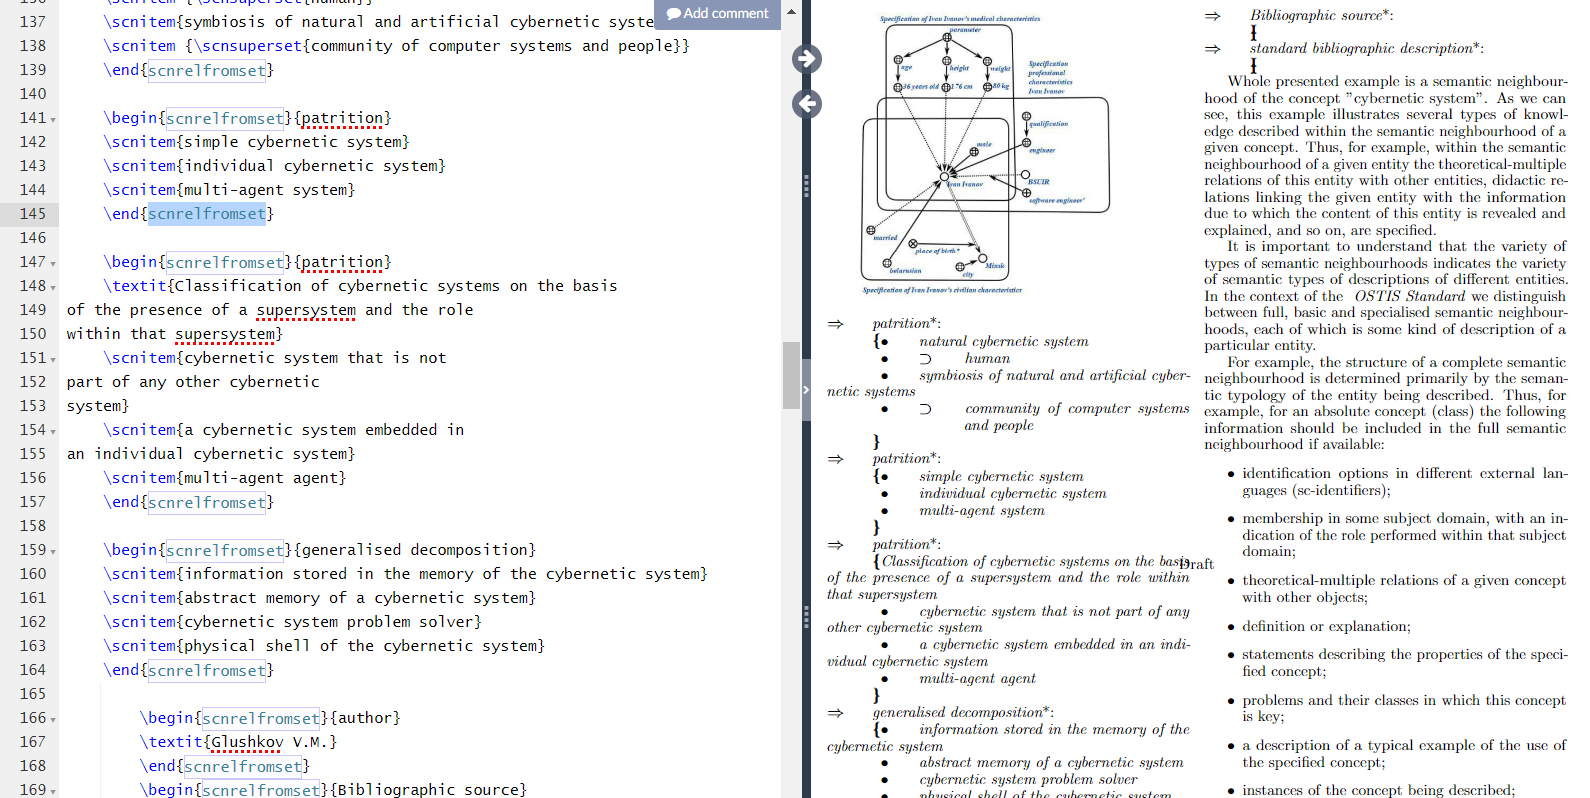
\includegraphics[width=0.75\linewidth]{image.png}
    \caption{ An example of the output of the response generation agent.}
    
\end{figure}


\begin{multicols}{2}


\normalsize
algorithmic approach that builds a tree of dependencies
between certain relations.\par
The actual generation of a natural language text is
proposed as a two-step process, whereby a large language
model generates the resulting text from an intermediate
representation.\par
Due to the preliminary character of our work, there
are certain limitations. Our approach does not discuss
linearization of graph-based formal texts in greater detail
apart from positing relatively straightforward schemata
to be used during translation. In fact, given that the
ultimate application of the module discussed here is
natural language dialog between humans and intelligent
systems, our proposed approach can be improved in three
different ways:

\begin{itemize}[noitemsep]%позволяет делать точки
\item Firstly, understanding natural language questions to
the system can be done using not a simple classifier
but rather a combination of syntactic and semantic
analysis modules that use a formalization of natural
language syntax and semantics.
\item Secondly, the linearization task can be solved in a
much more elaborate manner. This would require
formalization of a discourse structure model within
the knowledge base of an ostis-system. The model
can then be used to intelligently derive macro- and
microstructures of sc-texts to be translated into a natural language.
\item Finally, the actual translation of linearized sc-texts
into a natural language needs further elaboration.
An obvious improvement is to eliminate specific
rules (mappings) of translating sc-constructions into
certain predefined natural language verbalizations,
which would require designing a proper natural
language synthesis module.
\par
All of the above can be considered as potential directions for future research.
\end{itemize}

\centerline{Acknowledgment}

The authors would like to thank the research teams of
the Department of Intellectual Information Technologies
of Belarusian State University of Informatics and Radioelectronics and the Department of Linguistics Disciplines
and Cross-Cultural Communication of Brest State Technical University for their help and valuable comments.\par
\vspace{3mm}
\centerline{References}

\setcounter{page}{93}%добовляет нумерацию страниц

\cite{1} T. Yu, S. Zhang, and Y. Feng, “Truth-aware context selection:
Mitigating the hallucinations of large language models being
misled by untruthful contexts,” 2024. [Online]. Available:
https://api.semanticscholar.org/CorpusID:268364338
\cite{2} Y. Wu, N. Hu, S. Bi, G. Qi, J. Ren, A. Xie, and W. Song,
“Retrieve-rewrite-answer: A kg-to-text enhanced llms framework
for knowledge graph question answering,” 2023.

\end{multicols}

\begin{multicols}{2}
\scriptsize
\begin{thebiblieography}
    

\cite{3} V. Golenkov, Ed., Tehnologija kompleksnoj podderzhki
zhiznennogo cikla semanticheski sovmestimyh intellektual’nyh
komp’juternyh sistem novogo pokolenija [Technology of complex
life cycle support of semantically compatible intelligent computer
systems of new generation ]. Bestprint, 2023.\par

\cite{4} A. Goylo and S. Nikiforov, “Natural language interfaces of nextgeneration intelligent computer systems,” Open semantic technologies for intelligent systems, no. 6, pp. 209–216, 2022.\par
\cite{5} W. Mann and S. Thompson, “Rethorical structure theory: Toward
a functional theory of text organization,” Text, vol. 8, pp. 243–281,
01 1988.\par
\cite{6} E. H. Hovy, “Automated discourse generation using discourse
structure relations,” Artificial Intelligence, vol. 63, no. 1, pp.
341–385, 1993. [Online]. Available: https://www.sciencedirect.
com/science/article/pii/000437029390\par
\cite{7} W. Kintsch and T. A. van Dijk, “Toward a model of
text comprehension and production.” Psychological Review,
vol. 85, pp. 363–394, 1978. [Online]. Available: https://api.
semanticscholar.org/CorpusID:1825457\par
\cite{8} B. J. Grosz and C. L. Sidner, “Attention, intentions, and the
structure of discourse,” Computational Linguistics, vol. 12, no. 3,
pp. 175–204, 1986. [Online]. Available: https://aclanthology.org/
J86-3001\par
\cite{9} K. R. McKeown, “Discourse strategies for generating naturallanguage text,” Artificial Intelligence, vol. 27, no. 1, pp. 1–41,
1985. [Online]. Available: https://www.sciencedirect.com/science/
article/pii/000437028590\par
\cite{10} J. Liu, S. Cohen, and M. Lapata, “Text generation from discourse
representation structures,” 01 2021, pp. 397–415.\par
\cite{11} C. Wang, R. van Noord, A. Bisazza, and J. Bos, “Evaluating
text generation from discourse representation structures,” in
Proceedings of the 1st Workshop on Natural Language
Generation, Evaluation, and Metrics (GEM 2021), A. Bosselut,
E. Durmus, V. P. Gangal, S. Gehrmann, Y. Jernite, L. PerezBeltrachini, S. Shaikh, and W. Xu, Eds. Online: Association
for Computational Linguistics, Aug. 2021, pp. 73–83. [Online].
Available: https://aclanthology.org/2021.gem-1.8\par
\cite{12} C. Gardent, A. Shimorina, S. Narayan, and L. Perez-Beltrachini,
“The WebNLG challenge: Generating text from RDF data,”
in Proceedings of the 10th International Conference on
Natural Language Generation, J. M. Alonso, A. Bugarín, and
E. Reiter, Eds. Santiago de Compostela, Spain: Association for
Computational Linguistics, Sep. 2017, pp. 124–133. [Online].\par
\cite{13} J. Guan, X. Mao, C. Fan, Z. Liu, W. Ding, and M. Huang, “Long
text generation by modeling sentence-level and discourse-level
coherence,” in Proceedings of the 59th Annual Meeting of
the Association for Computational Linguistics and the 11th
International Joint Conference on Natural Language Processing
(Volume 1: Long Papers), C. Zong, F. Xia, W. Li, and
R. Navigli, Eds. Online: Association for Computational
Linguistics, Aug. 2021, pp. 6379–6393. [Online]. Available:
https://aclanthology.org/2021.acl-long.499\par
\cite{14} D. Shunkevich, “Hybrid problem solvers of intelligent computer
systems of a new generation,” Open semantic technologies for
intelligent systems, no. 6, pp. 119–144, 2022.\par
\cite{15} A. Goylo and S. Nikiforov, “Means of formal description of
syntax and denotational semantics of various languages in nextgeneration intelligent computer systems,” Open semantic technologies for intelligent systems, no. 6, pp. 99–118, 2022.\par
\cite{16} L. Shu, L. Luo, J. Hoskere, Y. Zhu, Y. Liu, S. Tong, J. Chen, and
L. Meng, “Rewritelm: An instruction-tuned large language model
for text rewriting,” 2023.\par
\cite{17} M. Kovalev, A. Kroshchanka, and V. Golovko, “Convergence and
integration of artificial neural networks with knowledge bases
in next-generation intelligent computer systems,” Open semantic
technologies for intelligent systems, no. 6, pp. 173–186, 2022.\par
\cite{18} V. V. Golenkov, N. A. Gulyakina, and D. V. Shunkevich,
“Klyuchevye problemy i strategicheskie tseli rabot v oblasti
iskusstvennogo intellekta [key problems and strategic goals of
research in the field of artificial intelligence],” 2023, pp. 9–13.\par
\cite{19} “ostis-metasystem repository,” Available at: https://github.com/
ostis-ai/ostis-metasystem, (accessed 2024, March).

\columnbreak



\scriptsize
20] “Rasa,” Available at: https://rasa.com/, (accessed 2024, March).\par
[21] “Wit AI,” Available at: https://wit.ai/, (accessed 2024, March).
\end{thebiblieography}

\begin{center}
    
\normalsize
\textbf{
\centerline { ГЕНЕРАЦИЯ}
\cennterline{ЕСТЕСТВЕННО-ЯЗЫКОВЫХ}
\centerline{ТЕКСТОВ ИЗ БАЗ ЗНАНИЙ}
\centrline{OSTIS-СИСТЕМ}}
\end{center}



\large
\centerline{ Гойло А. А. Никифоров С. А. Головко О. В.}\par
\vspace{2mm}
\normalsize
В статье описывается подход к генерации связных текстов
на естественном языке из фрагментов баз знаний ostis-систем. Описана архитектура абстрактного sc-агента трансляции фрагмента базы знаний в естественный язык. Задача
генерации естественно-языкового текста подрязделяется на
три подзадачи: фильтрация структуры, декомпозиция фрагмента базы знаний и генерация эквивалентного естественноязыкового текста. Предлагаются два способа линеаризации фрагментов базы знаний: использование заданной спецификации порядка элементов фрагмента и алгоритмический. Предлагается выполнять генерацию эквивалентного
естественно-языкового текста в два этапа. На первом этапе
формируется черновое естественно-языковое представление
на основе правил сопоставления конструкций sc-текстов с
соответствующими им естественно-языковыми формулировками. На втором этапе такое промежуточное представление
транслируется в связный естественно-языковой текст с использованием большой языковой модели. Описываются три
возможных применения предлагаемого подхода.\par

     \begin{flushright}
     Received 18.03.2024
 \end{flushright}
   
\newpage
\end{multicols}{2}

\centerline{\textbf{\huge{Principles of Building}}}\par
\centerline{\textbf{\huge{Intelligent Robotic Systems}}}




\begin{multicols}{2}

\centerline{\texttt{Aliaksandr Kroshchanka}}\par
\centerline{\textit{Brest State Technical University}}
\centerline{Brest, Belarus}
\centerline{kroschenko@gmail.com}
\vspace{10mm}
\footnotesize
\textbf{\textit{Abstract}—The paper proposes a concept for the building
of collaborative robotic systems using OSTIS technology.
The developed concept is based on the integration of robotic,
symbolic and neural network components. The main provisions of the approach are illustrated by the project of
a robotic system for sorting objects with specified characteristics. Recommendations are given on the application of
the proposed concept for the construction of collaborative
robotic systems in the context of the development of new
generation intelligent computer systems based on the use
of OSTIS technology.}\par
\textbf{\textit{Keywords}—OSTIS, collaborative robotics, hybrid intelligent systems, object detection, manipulators}
\vspace{2mm}

\centerline{\rom{1. }\space Introduction}
\vspace{2mm}
\normalsize
In modern collaborative robotic systems, robots follow
a set algorithm of actions, including the performance of
some predefined operations (e. g., grasping and moving
an object, positioning at a certain point, performing a certain operation on an object). Technically, the realization
of such actions does not cause difficulties in case of an
ideal workflow. However, there may be situations when
there are deviations from the established algorithm of
actions, for example, absence of an object in a given point
by the beginning of the operation, wrong type of object
or impossibility to perform the operation due to blocking
of moving parts, appearance of unauthorized persons in
the area of manipulator operation, etc. These problems
can be solved by using machine learning methods, in particular, neural networks. For example, a detector network
allows you to determine the type of object moving along
the conveyor, another model calculates the position of
the manipulator at the next moment of time depending
on the technical operation being performed, etc. However,
the use of only specialized auxiliary models, for example,
a computer vision model for detecting missing objects,
will not be able to help in the correct identification of the
place where objects of a given type can be located and
where, in case of absence of the object on the conveyor,
it will be necessary to deploy the manipulator to grab the
part. Information about important aspects of the manufacturing process, which is sufficiently variable, needs to be
systematically stored because the alternative — the need
for constant direct code editing in the context of changes\par
\columnbreak

\centerline{\texttt{Mikhail Kovalev}}\par
\centerline{\textit{Belarusian State University of}}
\centerline{Informatics and Radioelectronics}
\centerline{Minsk, Belarus}
\centerline{michail.kovalev7@gmail.com}
\vspace{5mm}



occurring to the robot — is unacceptable and, moreover,
can often lead to errors. In addition, the experience that
such systems may acquire during their operation is also
clearly important and needs to be properly represented
for reuse in other contexts and processes.\par
Thus, the development of principles and recommendations for the construction of intelligent robotic systems
is an urgent topic of research, because it allows to
streamline the process of developing such systems. The
use of modern tools for designing intelligent systems,
which undoubtedly includes OSTIS technology, allows
the representation and operation of knowledge, which is
a valuable resource in robotic systems.\par
The subsequent sections of the paper are organized
as follows: section II sets out the problem of building
knowledge-based robotics systems, in the same section
an overview of existing solutions is given; section III
describes the proposed concept for building intelligent
robotics systems; section IV describes the developed
prototype of an intelligent robotics system for sorting
objects of a given type; finally, section V summarizes the
main conclusions of the proposed concept and describes
the main conclusions of the intelligent robotics system
for sorting objects of a given type.
\normalsize
\vspace{2mm}

\centerline{\rom{2. } \space Problem formulation}
\vspace{2mm}

The idea of developing robotic systems based on the
use of knowledge bases has been widely investigated in
various works. For example, in [1], the authors give an
overview of knowledge bases used in robotic systems
to find missing tools. Emphasis is placed on finding
those objects without which further workflow continuation will not be possible. However, other applications\par
of knowledge bases are not indicated, in particular, the
possibility of using them for robot self-diagnosis, which
is an important function of such systems. Other studies
use knowledge bases (e. g., Cyc [2] or SUMO [3]) that
are not specific to robotics, which makes it difficult to
use such solutions in practice. One of the most promising
solutions at the moment is the KnowRob KB ( [4], [5]),
which is characterized by a developed ontological basis
for robotics.

 

\end{multicols}{2}
\end{document}
